\documentclass{beamer}

\mode<presentation>
{
  \usetheme{umbc1}
  \setbeamercovered{transparent}
}

\usepackage[english]{babel}
\usepackage[latin1]{inputenc}
\usepackage[T1]{fontenc}

\usepackage[]{datatool, filecontents}
\DTLsetseparator{=}
\DTLloaddb[noheader, keys={key,value}]{values}{./values.dat}
\newcommand{\var}[1]{\DTLfetch{values}{key}{#1}{value}}

\usepackage{tabularray}

\title[RMP v\var{version}]
{Robot Motion Planning}

\subtitle
{Configuration Space and Bug Algorithms}

\author[Narayanan]
{A.~Narayanan\inst{1}}

\institute[Technical University of Munich]
{
  \inst{1}
  Department of Informatics\\
}

\subject{Slides}

\AtBeginSubsection[]
{
  \begin{frame}<beamer>{Outline}
    \tableofcontents[currentsection,currentsubsection]
  \end{frame}
}

\begin{document}

\begin{frame}
  \titlepage
\end{frame}

\begin{frame}{Outline}
  \tableofcontents
\end{frame}


\section{Overview of Concepts in Motion Planning}

\subsection[Classification]{Classification}

  \begin{frame}{Classification by concepts}
      \centering
    \begin{table}
      \begin{tblr}{c|Q[3cm,valign=m]|Q[3.5cm,valign=m]}
          Task & Robot & Algorithm \\
          \hline 
          Navigate & Configuration space, degree of freedom & Optimal/nonoptimal motions \\
          Map & Kinematic/dynamic & Computational complexity \\
          Cover & Omnidirectional or motion constraints & Completeness (resolution, probabilistic) \\
          Localize &  & Online/offline Sensor-based/world model \\
      \end{tblr}
    \end{table}
  \end{frame}

  \begin{frame}{Classification by Task}
    \begin{itemize}
    \item
    The most important characterization of a motion planner is according to the problem
    it solves. \pause The four major tasks are \texttt{navigation},  \texttt{coverage},  \texttt{localization}, and
    \texttt{mapping}.
    \pause
    \item \textbf{Navigation} is the problem of finding a collision-free motion for the robot system from one configuration (or state) to another. \pause
    \item \textbf{Coverage} is the problem of passing a sensor or tool over all points in a space, such as in demining or painting. \pause
    \item \textbf{Localization} is the problem of using a map to interpret sensor data to determine the configuration of the robot. \pause
    \item \textbf{Mapping} is the problem of exploring and sensing an unknown environment to construct a representation that is useful for navigation, coverage, or localization. \pause
    \item Localization and mapping can be combined, as in SLAM.
    \end{itemize}
  \end{frame}

  \begin{frame}{Classification by Robot Properties}
    Todo\dots
  \end{frame}

  \begin{frame}{Classification by Algorithm}
    Todo\dots
  \end{frame}

\subsection[Notations]{Mathematical Notations}

\begin{frame}{Mathematical Notations}
  
  \begin{columns}
    \begin{column}{0.5\textwidth}
      \begin{itemize}
        \item $\mathcal{W}$  - Workspace \pause
        \item $\mathcal{W} \mathcal{O}_{i} $ - the $i^{th}$ Obstacle \pause
        \item $\mathcal{W}_{free}$ - Free Workspace \pause
        \item $\mathcal{Q}$ - Configuration Space \pause
        \item $\mathcal{Q} \mathcal{O}_{i} $ - the $i^{th}$ Obstacle in Config Space \pause
        \item $R(q)$ - Set of points in ambient space occupied by the robot at config q
        \end{itemize}
    \end{column}
    \begin{column}{0.5\textwidth}  %%<--- here
        \begin{center}
          \begin{figure}
            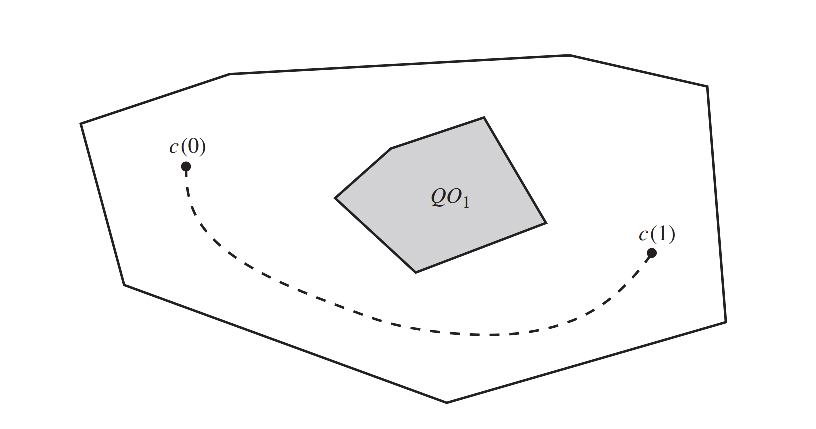
\includegraphics[width=60mm]{fig/fig_01.png}
            \caption{A path.}
            \label{fig:fig01}
          \end{figure}
         \end{center}
    \end{column}
    \end{columns}
\end{frame}

\section[Bug Algorithms]{Bug Algorithms}

\subsection[Assumptions]{Assumptions}

\begin{frame}{Assumptions}
  \begin{itemize}
    \item Assume a point robot
    \item Assume a zero range sensor
    \item Assume the robot can measure $d(x,y)$ between any $x \in \mathbb{R}^{2} $ and $y \in \mathbb{R}^{2}$ in a bounded workspace
  \end{itemize}
\end{frame}

\subsection[Bug 0]{Bug 0 Algorithm}

\subsection[Bug 1]{Bug 1 Algorithm}

\subsection[Bug 2]{Bug 2 Algorithm}

\subsection[Tangential Bug]{Tangential Bug Algorithm}

\section[Configuration Space]{Configuration Space}

\section*{Summary}

\begin{frame}{Summary}

  \begin{itemize}
  \item
    The \alert{first main message} of your talk in one or two lines.
  \item
    The \alert{second main message} of your talk in one or two lines.
  \item
    Perhaps a \alert{third message}, but not more than that.
  \end{itemize}
  
  \vskip0pt plus.5fill
  \begin{itemize}
  \item
    Outlook
    \begin{itemize}
    \item
      Something you haven't solved.
    \item
      Something else you haven't solved.
    \end{itemize}
  \end{itemize}
\end{frame}

\end{document}
